% !TeX root = er.tex

\chapter{Navegação local: Prevenção de Obstáculos}\label{ch.obstacle}

Um robô móvel deve {navigar} de um ponto a outro de seu ambiente. Esta pode ser uma tarefa simples, por exemplo, se um robô pode seguir uma linha desobstruída no chão de um armazém (Sect.~\ref{s.line}), mas a tarefa torna-se mais difícil em ambientes desconhecidos e complexos como um rover explorando a superfície de Marte ou um submersível explorando uma cadeia de montanhas submarinas. Mesmo um carro que viaja por uma estrada precisa lidar com outros carros, obstáculos na estrada, passadeiras para pedestres, construção de estradas, e assim por diante. 

A navegação de um carro que se auto dirige pode ser dividida em duas tarefas: Há a tarefa de alto nível de encontrar um caminho entre uma posição de partida e uma posição de objetivo. Antes do desenvolvimento de sistemas modernos de computador, encontrar um caminho exigia o estudo de um mapa ou a pergunta de direções. Agora existem aplicativos smartphone que tomam uma posição inicial e uma posição de objetivo e computam os caminhos entre as duas posições. Se o aplicativo receber dados em tempo real sobre as condições de tráfego, ele pode sugerir qual caminho o levará ao seu objetivo no menor tempo possível. O caminho pode ser computado offline, ou, se você tiver um sistema GPS que possa determinar sua posição atual, o caminho pode ser encontrado em tempo real e atualizado para levar em conta as condições de mudança.

Um carro que dirige sozinho também deve realizar a tarefa de nível inferior de adaptar seu comportamento ao ambiente: parar para um pedestre em uma faixa de pedestres, virar em cruzamentos, evitar obstáculos na estrada, etc. Embora a busca de caminhos de alto nível possa ser feita uma vez antes da viagem (ou a cada poucos minutos), a tarefa de evitar obstáculos de baixo nível deve ser realizada com freqüência, pois o carro nunca sabe quando um pedestre irá pular na estrada ou quando o carro que está seguindo irá frear de repente.

A seção~\ref{s.obstacle-avoidance} examina a tarefa de baixo nível de evitar obstáculos. A seção~\ref{s.no-localization} mostra como um robô pode reconhecer marcas enquanto segue uma linha para que ele saiba quando atingiu seu objetivo. As seções~\{sref{s.ants}--\ref{s.fsm-ants} demonstram um comportamento de nível superior: encontrar um caminho sem um mapa do ambiente. Isto é feito por analogia com uma colônia de formigas que localiza uma fonte de alimento e comunica sua localização a todos os membros da colônia.

\section{Evitar obstáculos}\label{s.obstacle-avoidance}

Os algoritmos apresentados até agora têm se concentrado na detecção de objetos e no movimento em direção a eles. Quando um robô se move em direção a um objetivo é provável que encontre objetos adicionais chamados \emph{obstacles} que bloqueiam o caminho e impedem o robô de alcançar seu objetivo. Supomos que o robô é capaz de detectar se há um caminho desobstruído para a meta, por exemplo, detectando uma luz sobre a meta. Esta seção descreve três algoritmos para evitar obstáculos, onde os obstáculos são paredes que bloqueiam o movimento do robô:
\begin{itemize}
\item Uma parede simples seguindo um algoritmo, que infelizmente não funcionará se houver múltiplos obstáculos no ambiente.
\item Um algoritmo que pode evitar múltiplos obstáculos, mas deve conhecer a direção geral do objetivo (talvez a partir de seu sistema GPS). Infelizmente, alguns obstáculos podem fazer com que o robô fique preso em um loop.
\item O algoritmo Pledge é uma pequena modificação do segundo que supera este comportamento errôneo.
\end{itemize}
Os algoritmos utilizarão as expressões condicionais abstratas \p{wall-ahead} e \p{wall-right}, que são verdadeiras se houver uma parede próxima à frente ou à direita do robô. O primeiro algoritmo também utilizará a expressão condicional \p{corner-direita}, que é verdadeira se o robô estiver se movendo em torno de um obstáculo e sentir um canto à sua direita. Há várias maneiras de implementar estas expressões que buscamos na Activity~\ref{act.wall-expressions}.

\begin{framed}
\act{Expressões condicionais para o seguimento de muros}{wall-expressions}
\begin{itemize}
\item Implemente a expressão condicional \p{wall-ahead} usando uma proximidade horizontal ou um sensor de toque.
\item Implemente a expressão condicional \p{wall-right}. Isto é fácil de fazer com um sensor montado à direita do robô, ou com um sensor de distância rotativo. Se você tiver apenas um sensor de proximidade voltado para frente, você pode fazer o robô girar ligeiramente para a direita, detectar a parede, se houver, e então girar novamente para trás.
\item Implemente a expressão condicional \p{corner-direita}. Isto pode ser implementado como uma extensão da \p{wall-direita}. Quando o valor da palavra \p{parede direita} mudar de verdadeiro para falso, faça uma curva curta à direita e verifique se a palavra "parede direita" se torna verdadeira novamente.
\end{itemize}
\end{framed}

\subsection{Seguimento de parede}

A figura~\ref{fig.wall-following-simple} mostra um robô realizando o seguimento da parede mantendo sua posição para que a parede fique à sua direita (Algoritmo~\ref{alg.wall-following-simple}). Se uma parede for detectada à frente, o robô vira à esquerda para que a parede fique à sua direita. Se for detectada uma parede para a direita, o robô continua se movendo ao longo da parede. Se for detectada uma curva, o robô vira à direita para continuar se movendo ao redor do obstáculo. Ao mesmo tempo, o robô procura continuamente o objetivo (ponto negro). Quando detecta a meta, o robô se move diretamente em direção a ela.

\begin{figure}
\begin{center}
\begin{tikzpicture}[scale=.7]
\draw[fill,color=gray] (4,0) rectangle +(4,.8);
\draw[fill,color=gray] (5,0) rectangle +(.8,-1);
\pic[rotate=90,scale=.5] at (7,-3) { robot };
\draw[fill] (6,4) node[right,xshift=4pt] {\p{Goal}} circle[radius=4pt];
\draw[->] (7,-2) -- ++(90:1.8) -- ++(180:1) -- ++(-90:1) -- ++(180:1.2) -- ++(90:1) -- ++(180:1) -- ++(90:1.2) coordinate(corner);
\draw[dashed,->] (corner) -- (5.9,3.9);
\path (-.3,0);  % Extra space so arrow isn't chopped
\end{tikzpicture}
\caption{Seguimento de parede}\label{fig.wall-following-simple}
\end{center}
\end{figure}

\begin{figure}
\begin{alg}{Seguimento simples da parede}{wall-following-simple}
\hline
\stl{}&while not-at-goal&\\
\stl{}&\idc{}if goal-detected&\\
\stl{}&\idc{}\idc{}move towards goal&\\
\stl{}&\idc{}else if wall-ahead&\\
\stl{}&\idc{}\idc{}turn left&\\
\stl{}&\idc{}else if corner-right&\\
\stl{}&\idc{}\idc{}turn right&\\
\stl{}&\idc{}else if wall-right&\\
\stl{}&\idc{}\idc{}move forward&\\
\stl{}&\idc{}else&\\
\stl{}&\idc{}\idc{}move forward&\\
\end{alg}
\end{figure}

Infelizmente, o Algorithm~\ref{alg.wall-following-simple} nem sempre funciona corretamente.  Fig.~\ref{fig.wall-following-simple-bug} mostra uma configuração com \emph{dois} obstáculos entre o robô e o objetivo. O robô nunca detectará o objetivo, então ele se moverá indefinidamente em torno do primeiro obstáculo.


\begin{framed}
\act{Seguimento simples da parede}{simple-wall-following}
\begin{itemize}
\item Implementar o Algoritmo~\ref{alg.wall-following-simple} e verificar se ele demonstra os comportamentos mostrados em Figs.~\ref{fig.wall-following-simple}, \ref{fig.wall-following-simple-bug}.
\end{itemize}
\end{framed}

\begin{figure}
\begin{center}
\begin{tikzpicture}[scale=.8]
\draw[fill,color=gray] (4,0) rectangle +(4,.8);
\draw[fill,color=gray] (5,0) rectangle +(.8,-1);
\draw[fill,color=gray] (0,2) rectangle +(9,.8);
\draw[fill,color=gray] (1.5,2) rectangle +(.8,-1);
\pic[rotate=90,scale=.5] at (7,-3) { robot };
\draw[fill] (6,4) node[right,xshift=4pt] {\p{Objetivo}} circle[radius=4pt];
\draw[->] (7,-2) -- ++(90:1.8) -- ++(180:1) -- ++(-90:1) -- ++(180:1.2) -- ++(90:1) -- ++(180:1) -- ++(90:1.2) coordinate(corner) -- ++(0:4.4) -- ++(-90:1.2) -- ++(180:1);
\draw[dashed,->] (corner) -- (5.9,3.9);
\path (-.3,0);  % Extra space so arrow isn't chopped
\end{tikzpicture}
\caption{O simples seguimento da parede nem sempre permite que o robô atinja o objetivo}\label{fig.wall-following-simple-bug}
\end{center}
\end{figure}

\subsection{Parede seguindo com direção}

O problema com o Algorithm~\ref{alg.wall-following-simple} é que ele é um algoritmo local que só olha para seu ambiente imediato e não leva em conta o fato de que o algoritmo de navegação de nível superior sabe aproximadamente a direção que o robô deve tomar para alcançar o objetivo. A figura~\ref{fig.wall-following-direction} mostra o comportamento de um robô que "sabe" que o objetivo está em algum lugar ao norte, então o robô se move a uma direção de $0^\circ$ em relação ao norte. O algoritmo de seguir a parede só é utilizado se o robô não puder se mover para o norte.

\begin{figure}
\begin{center}
\begin{tikzpicture}[scale=.7]
\draw[fill,color=gray] (4,0) rectangle +(4,.8);
\draw[fill,color=gray] (5,0) rectangle +(.8,-1);
\draw[fill,color=gray] (0,2) rectangle +(9,.8);
\draw[fill,color=gray] (1.5,2) rectangle +(.8,-1);
\pic[rotate=90,scale=.5] at (7,-3) { robot };
\draw[fill] (6,4) node[right,xshift=4pt] {\p{Objetivo}} circle[radius=4pt];
\draw[->] (7,-2) -- ++(90:1.8) -- ++(180:1) -- ++(-90:1) -- ++(180:1.2) -- ++(90:1) -- ++(180:1) -- ++(90:2) -- ++(180:1.3) -- ++(-90:1) -- ++(180:1.2) -- ++(90:1) -- ++(180:1.5) -- ++(90:1.4) coordinate(corner);
\draw[dashed,->] (corner) -- (5.8,4);
\path (-.3,0);  % Extra space so arrow isn't chopped
\end{tikzpicture}
\caption{Parede seguindo com direção}\label{fig.wall-following-direction}
\end{center}
\end{figure}

Algoritmo~\ref{alg.wall-follow} é semelhante ao algoritmo anterior, exceto por sua preferência de se mover para o norte, se possível. Utiliza uma variável \p{título} para lembrar seu título atual à medida que se move em torno do obstáculo. Quando o \p{título} está novamente ao norte (um múltiplo de $360^\circ$), o robô avança em vez de procurar por um canto.

\begin{figure}
\begin{alg}{Seguimento de parede}{wall-follow}
&\idv{}integer heading \ass $0^\circ$&\\
\hline
\stl{}&while not-at-goal&\\
\stl{}&\idc{}if goal-detected&\\
\stl{}&\idc{}\idc{}move towards goal&\\
\stl{}&\idc{}else if wall-ahead&\\
\stl{}&\idc{}\idc{}turn left&\\
\stl{}&\idc{}\idc{}heading \ass heading $+\: 90^\circ$&\\
\stl{}&\idc{}else if corner-right&\\
\stl{}&\idc{}\idc{}if heading $=$ multiple of $360^\circ$&\\
\stl{}&\idc{}\idc{}\idc{}move forward&\\
\stl{}&\idc{}\idc{}else&\\
\stl{}&\idc{}\idc{}\idc{}turn right&\\
\stl{}&\idc{}\idc{}\idc{}heading \ass heading $-\: 90^\circ$&\\
\stl{}&\idc{}else if wall-right&\\
\stl{}&\idc{}\idc{}move forward&\\
\stl{}&\idc{}else&\\
\stl{}&\idc{}\idc{}move forward&\\
\end{alg}
\end{figure}

Infelizmente, o algoritmo pode falhar quando confrontado com um obstáculo em forma de "grifo" (Fig.~\ref{fig.wall-direction-bug}). Depois de fazer quatro voltas à esquerda, seu título é $360^\circ$ (também ao norte, um múltiplo de $360^\circ$) e continua avançando, encontrando e seguindo a parede uma e outra vez.

\begin{figure}
\begin{center}
\begin{tikzpicture}[scale=.7]
\draw[fill,color=gray] (0,0) rectangle +(4,.8);
\draw[fill,color=gray] (3.2,0) rectangle +(.8,1.5);
\draw[fill,color=gray] (0,0) rectangle +(.8,4);
\draw[fill,color=gray] (0,3.2) rectangle +(6,.8);
\pic[rotate=90,scale=.5] at (5.2,.3) { robot };
\draw[->] (5.2,1.1) -- ++(90:1.9) -- ++(180:4.2) -- ++(-90:2) -- ++(0:2) -- ++(90:1.6);
\draw[->,thick] (-1,1) -- node[left,xshift=-4pt] {\p{Objetivo}} +(0,2);
\end{tikzpicture}
\caption{Por que seguir a parede com direção nem sempre funciona}\label{fig.wall-direction-bug}
\end{center}
\end{figure}

\begin{framed}
\act{Parede seguindo com direção}{wall-following}
\begin{itemize}
\item Implemente o algoritmo de seguimento de parede com direção e verifique se ele demonstra o comportamento mostrado na Fig.~\ref{fig.wall-direction-bug}.
\item Executar o algoritmo de seguimento de parede simples (Algoritmo~\ref{alg.wall-following-simple}) com um obstáculo em forma de grifo (G). O que acontece? Isto afeta nossa afirmação de que este algoritmo não é adequado para evitar obstáculos?
\end{itemize}
\end{framed}

\subsection{O algoritmo Pledge}

O algoritmo Pledge modifica a linha~8 da parede seguindo o algoritmo para:
\begin{quote}
\normalsize \p{if heading $= 0^\circ$}
\end{quote}
O robô avança somente quando seu título cumulativo é igual a $0^\circ$ e não quando está se movendo para o norte - um título que é um múltiplo de $360^\circ$. O robô agora evita o obstáculo em forma de ``G'' (Fig.~\ref{fig.wall-following-pledge}): quando encontra o canto (ponto negro), ele está se movendo para o norte, mas seu rumo é de $360^\circ$ depois de quatro voltas à esquerda. Embora $360^\circ$ seja um múltiplo de $360^\circ$, ele não é igual a $0^\circ$. Portanto, o robô continua a seguir a parede até quatro curvas à direita subtraindo $360$, de modo que o total da direção é de $0^\circ$.

\begin{figure}
\begin{center}
\begin{tikzpicture}[scale=.7]
\draw[fill,color=gray] (0,0) rectangle +(4,.8);
\draw[fill,color=gray] (3.2,0) rectangle +(.8,1.5);
\draw[fill,color=gray] (0,0) rectangle +(.8,4);
\draw[fill,color=gray] (0,3.2) rectangle +(6,.8);
\pic[rotate=90,scale=.5] at (5.2,.3) { robot };
\draw[->] (5.2,1.1) -- ++(90:1.9) -- ++(180:4.2) -- ++(-90:2) -- ++(0:2) -- ++(90:.7) -- ++(0:1.2) -- ++(-90:1.9) -- ++(180:4.4) -- ++(90:4.5);
\fill (3.2,1.5) circle [radius=3pt];
\draw[->,thick] (-1,1) -- node[left,xshift=-4pt] {\p{Objetivo}} +(0,2);
\path (-.3,0);  % Extra space so arrow isn't chopped
\end{tikzpicture}
\caption{Algoritmo de juramento para acompanhamento de parede}\label{fig.wall-following-pledge}
\end{center}
\end{figure}

\begin{framed}
\act{Algoritmo de Pledge}{pledge-algorithm}
\begin{itemize}
\item Implementar o algoritmo Pledge e verificar se ele demonstra o comportamento mostrado em Fig.~\ref{fig.wall-following-pledge}.
\end{itemize}
\end{framed}

\section{Seguindo uma linha com um código}\label{s.no-localization}

Voltemos à tarefa de encontrar um caminho para um objetivo. Se o caminho é marcado por uma linha no chão, a linha seguindo os algoritmos (Sect.~\ref{s.line}) pode guiar um robô dentro do ambiente, mas a linha seguindo não é navegação. Para navegar de uma posição para outra também precisamos de um algoritmo de localização para que o robô saiba quando atingiu seus objetivos. Não precisamos de um algoritmo de localização contínua como os do Chap.~\ref{ch.local}, precisamos apenas conhecer posições na linha que facilitem o cumprimento da tarefa. Isto é semelhante à navegação ao dirigir: você só precisa saber sobre intercâmbios, cruzamentos, marcos importantes, etc., para saber onde você está. Entre tais posições, você pode simplesmente seguir a estrada.

A navegação sem localização contínua pode ser implementada através da leitura de um código colocado no piso próximo à linha. A figura~\ref{fig.code-line} mostra um robô com dois sensores de solo: o da esquerda detecta a linha e o da direita detecta o código. Abaixo do robô há um gráfico do sinal retornado pelo sensor direito.

\begin{figure}
\begin{center}
\begin{tikzpicture}
\draw[fill,lightgray] (-1,-4mm) rectangle +(8,5mm);
\pic[scale=1.2] at (0,-7mm) { robot2 };
\draw[fill,lightgray] (20mm,-14mm) rectangle +(4mm,6mm);
\draw[fill,lightgray] (30mm,-14mm) rectangle +(8mm,6mm);
\draw[fill,lightgray] (50mm,-14mm) rectangle +(4mm,6mm);
\draw[very thick,rounded corners] (-10mm,-30mm) -- ++(29mm,0mm) -- ++(2mm,8mm) -- ++(3mm,0mm) -- ++(2mm,-8mm) -- ++(3mm,0mm) -- ++(2mm,8mm) -- ++(6mm,0mm) -- ++(2mm,-8mm) -- ++(10mm,0mm) -- ++(2mm,8mm) -- ++(3mm,0mm) -- ++(2mm,-8mm) -- ++(12mm,0mm);
\node at (4mm,-26mm) {\p{saída correta do sensor}}; 
\end{tikzpicture}
\end{center}
\caption{Um robô seguindo uma linha usando seu sensor esquerdo e lendo um código com seu sensor direito}\label{fig.code-line}
\end{figure}

\begin{framed}
\act{Linha seguinte durante a leitura de um código}{line-coded}
\begin{itemize}
\item Implementar linha seguinte com leitura de código como mostrado em Fig.~\ref{fig.code-line}.
\item Escreva um programa que faz com que um robô siga um caminho.
\item Colocar marcas que codificam valores ao lado do caminho. O robô deve exibir estes valores (usando luz, som ou uma tela) quando se mover sobre os códigos.
\end{itemize}
\end{framed}

\begin{framed}
\act{Linha circular seguinte durante a leitura de um código}{line-coded-circular}
\begin{itemize}
\item Implementar um relógio usando dois robôs, um para os minutos e outro para as horas (Fig.~\ref{fig.line-clock}).
\item Uma implementação alternativa seria fazer com que os dois robôs se movessem em velocidades diferentes para que um complete uma revolução em uma hora e o outro complete uma revolução em um dia. Discutir a diferença entre as implementações.
\end{itemize}
\end{framed}

\begin{figure}
\begin{center}
\begin{tikzpicture}[scale=.8]
\begin{scope}[lightgray,line width=2.5mm]
\draw (0,0) circle[radius=44mm];
\foreach \n in {12, 1, 2, 3, 4, 5, 6, 7, 8, 9, 10, 11} {
  \node at (\n*30:51mm) [rectangle,fill,draw,rotate=\n*30] {};
  \node[black] at (90-\n*30:56mm) {\p{\n}};
}
\draw[lightgray] (0,0) circle[radius=20mm];
\foreach \n in {12, 1, 2, 3, 4, 5, 6, 7, 8, 9, 10, 11} {
  \node at (\n*30:27mm) [rectangle,fill,draw,rotate=\n*30] {};
  \node[black] at (90-\n*30:32mm) {\p{\n}};
}
\node at (0,0) [rectangle,fill,draw,minimum width=8mm,inner sep=1pt] {};
\node at (0,0) [rectangle,fill,draw,minimum height=8mm,inner sep=1pt] {};
\end{scope}
\pic[scale=.7,rotate=279] at (15:23mm) { robot2 };
\pic[scale=.7,rotate=-50] at (46:48mm) { robot2 };
\end{tikzpicture}
\end{center}
\caption{Um relógio robótico: um robô indica a hora e o outro indica o minuto}\label{fig.line-clock}
\end{figure}

\section{Formigas em busca de uma fonte de alimento}\label{s.ants}

Voltemos agora ao algoritmo de alto nível de encontrar um caminho. Se houver uma linha e um mecanismo de localização como um código, a abordagem da seção anterior pode ser usada. Entretanto, mesmo que uma linha não exista, um robô pode ser capaz de \emph{criar} sua própria linha. O aspecto interessante deste método é que o robô não precisa saber sua localização no ambiente, por exemplo, usando um GPS; ao invés disso, ele usa pontos de referência no próprio ambiente para navegação. O algoritmo será apresentado dentro do contexto do mundo real das formigas em busca de alimentos:

\begin{quote}
\normalsize Existe um ninho de formigas. As formigas buscam aleatoriamente uma fonte de alimento. Quando uma formiga encontra alimento, ela retorna diretamente ao ninho usando pontos de referência e sua memória do caminho que tomou do ninho. Durante a viagem de retorno ao ninho com o alimento, as formigas depositam produtos químicos chamados \emph{pheromones}. Conforme mais e mais formigas encontram a fonte de alimento e retornam ao ninho, a trilha acumula mais feromônios do que as outras áreas que as formigas visitam. Eventualmente, a quantidade de feromônios na trilha será tão forte que as formigas poderão seguir um caminho direto do ninho até a fonte de alimento.
\end{quote}

A figura~\ref{fig.ant-nest-food} mostra o ninho de formigas no canto inferior esquerdo representado como uma luz que permite que as formigas encontrem facilmente o caminho de volta para o ninho. A mancha escura é a fonte de alimento. A figura~\ref{fig.ant-nest-food-trail} mostra três trilhas aleatórias que eventualmente descobrem a fonte de alimento; então as formigas retornam diretamente ao ninho, deixando três linhas retas de feromônios. Esta concentração pode ser usada posteriormente para encontrar a fonte de alimento diretamente.

\begin{figure}
\begin{minipage}{.45\textwidth}
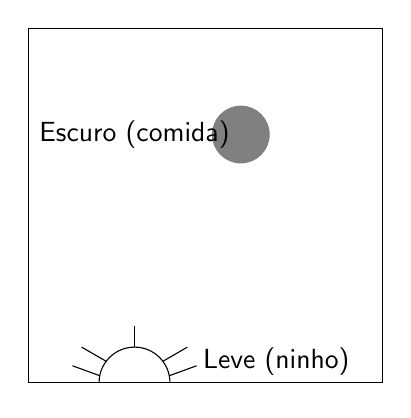
\begin{tikzpicture}[scale=.9]
% Light and dark with labels
\draw (0,0) -- (5,0) -- (5,5) -- (0,5) -- cycle;
\draw (2,0) arc[start angle=0, end angle=180, radius=5mm];
\node at (3.5,.3) {\textsf{Leve (ninho)}};
\draw (19mm,3mm) -- +(30:4mm);
\draw (20mm,1mm) -- +(20:4mm);
\draw (11mm,3mm) -- +(150:4mm);
\draw (10mm,1mm) -- +(160:4mm);
\draw (15mm,5mm) -- (15mm,8mm);
\draw[fill,gray] (3,3.5) circle[radius=4mm];
\node at (1.5,3.5) {\textsf{Escuro (comida)}};
\path (0,-.1) -- (5,-.1); % To prevent truncation
\end{tikzpicture}
\caption{O ninho das formigas e a fonte de alimento}\label{fig.ant-nest-food}
\end{minipage}
\hspace{\fill}
\begin{minipage}{.45\textwidth}
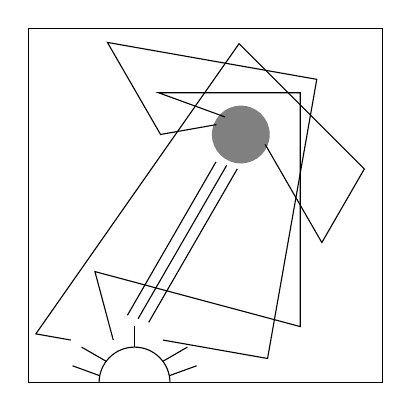
\begin{tikzpicture}[scale=.9]
\draw (0,0) -- (5,0) -- (5,5) -- (0,5) -- cycle;
\draw (2,0) arc[start angle=0, end angle=180, radius=5mm];
\draw (19mm,3mm) -- +(30:4mm);
\draw (20mm,1mm) -- +(20:4mm);
\draw (11mm,3mm) -- +(150:4mm);
\draw (10mm,1mm) -- +(160:4mm);
\draw (15mm,5mm) -- (15mm,8mm);
\draw[fill,gray] (3,3.5) circle[radius=4mm];
% Straight lines between light and dark
\begin{scope}[xshift=-1mm,yshift=2mm]
%\draw (13.5mm,8mm) -- +(60:2.5);
\draw (15mm,7.5mm) -- +(60:2.5);
\draw (16.5mm,7mm) -- +(60:2.5);
\draw (18mm,6.5mm) -- +(60:2.5);
\end{scope}
% Random lines between light and dark
\draw (19mm,6mm) -- ++(-10:15mm) -- ++(80:40mm) -- ++(170:30mm) -- ++(-60:15mm) -- ++(10:8mm);
\draw (12mm,6mm) -- ++(-75:-10mm) -- ++(-15:30mm) -- ++(90:33mm) -- ++(180:20mm) -- ++(-20:10mm);
\draw (6mm,6mm) -- ++(170:5mm) -- ++(55:50mm) -- ++(-45:25mm) -- ++(-120:12mm) -- ++(120:16mm);
\path (0,-.1) -- (5,-.1); % To prevent truncation
\end{tikzpicture}
\caption{As feromonas criam uma trilha}\label{fig.ant-nest-food-trail}
\end{minipage}
\end{figure}

%\begin{figure}
%\subfigures
%\begin{minipage}{\textwidth}
%\leftfigure[c]{
%\begin{tikzpicture}
%% Light and dark with labels
%\draw (0,0) -- (5,0) -- (5,5) -- (0,5) -- cycle;
%\draw (2,0) arc[start angle=0, end angle=180, radius=5mm];
%\node at (3.5,.3) {\textsf{Light (nest)}};
%\draw (19mm,3mm) -- +(30:4mm);
%\draw (20mm,1mm) -- +(20:4mm);
%\draw (11mm,3mm) -- +(150:4mm);
%\draw (10mm,1mm) -- +(160:4mm);
%\draw (15mm,5mm) -- (15mm,8mm);
%\draw[fill,gray] (3,3.5) circle[radius=4mm];
%\node at (1.5,3.5) {\textsf{Dark (food)}};
%\path (0,-.1) -- (5,-.1); % To prevent truncation
%\end{tikzpicture}
%}
%\hspace{\fill}
%\rightfigure[c]{
%\begin{tikzpicture}
%\draw (0,0) -- (5,0) -- (5,5) -- (0,5) -- cycle;
%\draw (2,0) arc[start angle=0, end angle=180, radius=5mm];
%\draw (19mm,3mm) -- +(30:4mm);
%\draw (20mm,1mm) -- +(20:4mm);
%\draw (11mm,3mm) -- +(150:4mm);
%\draw (10mm,1mm) -- +(160:4mm);
%\draw (15mm,5mm) -- (15mm,8mm);
%\draw[fill,gray] (3,3.5) circle[radius=4mm];
%% Straight lines between light and dark
%\begin{scope}[xshift=-1mm,yshift=2mm]
%%\draw (13.5mm,8mm) -- +(60:2.5);
%\draw (15mm,7.5mm) -- +(60:2.5);
%\draw (16.5mm,7mm) -- +(60:2.5);
%\draw (18mm,6.5mm) -- +(60:2.5);
%\end{scope}
%% Random lines between light and dark
%\draw (19mm,6mm) -- ++(-10:15mm) -- ++(80:40mm) -- ++(170:30mm) -- ++(-60:15mm) -- ++(10:8mm);
%\draw (12mm,6mm) -- ++(-75:-10mm) -- ++(-15:30mm) -- ++(90:33mm) -- ++(180:20mm) -- ++(-20:10mm);
%\draw (6mm,6mm) -- ++(170:5mm) -- ++(55:50mm) -- ++(-45:25mm) -- ++(-120:12mm) -- ++(120:16mm);
%\path (0,-.1) -- (5,-.1); % To prevent truncation
%\end{tikzpicture}
%}
%\leftcaption{The ants' nest and the food source\label{fig.ant-nest-food}}
%\rightcaption{Pheromones create a trail\label{fig.ant-nest-food-trail}}
%\end{minipage}
%\end{figure}

O comportamento semelhante ao de uma formiga pode ser implementado por um robô.\label{s.ant-like-algo} Como na Fig.~\ref{fig.ant-nest-food}, há uma fonte de alimento e um ninho. A fonte de alimento será representada por uma mancha escura que pode ser facilmente detectada por um sensor terrestre no robô. Os sensores de proximidade do robô são usados para detectar as paredes da área. Atividade~\ref{act.locate-nest} sugere dois métodos de representação do ninho que dependem dos sensores adicionais que seu robô possui.

\begin{framed}
\act{Localização do ninho}{locate-nest}
\begin{itemize}
\item Implementar um programa que faz com que o robô se mova para o ninho, não importa onde ele seja colocado na área.
\item Acelerômetros: Monte a área em uma encosta tal que um canto, o ninho, esteja no ponto mais baixo da área. 
\item Sensor de luz: O ninho é representado por uma fonte de luz que pode ser detectada pelo sensor de luz, independentemente da posição e do rumo do robô. Se o sensor de luz for fixo e puder detectar a luz somente de uma determinada direção, o robô terá que girar para localizar a fonte de luz.
\end{itemize}
\end{framed}

Simular as feromonas cobrindo a área com uma folha de papel branco e prendendo um marcador preto ao robô para que ele desenhe uma linha onde quer que ele se mova. Um sensor de terra detecta as marcas na área. A figura~\ref{fig.ant-result} mostra as linhas resultantes do comportamento de um robô executando o algoritmo. A atividade~\ref{act.high-density} pede que você explore a capacidade do robô de detectar áreas que têm uma alta densidade de linhas.

\begin{figure}
\begin{center}
\includegraphics[width=.8\textwidth]{density-map-0}
\end{center}
\caption{Um robô que simula feromônios de formigas}\label{fig.ant-result}
\end{figure}

\begin{framed}
\act{Sensoriamento de áreas de alta densidade}{high-density}
\begin{itemize}
\item Na seita Sect.~\ref{s.no-gradient} observamos que os sensores não sentem um único ponto geométrico, mas têm uma abertura que lê uma área relativamente grande, talvez até mesmo um centímetro quadrado (Fig.~\ref{fig.no-gradient}). Experimente com seu sensor de solo para ver como as leituras retornadas pelo sensor dependem da largura da linha. Você pode chegar a alguma conclusão sobre a largura ideal do marcador? Se for muito fino, o rastro não será detectado e se for muito grosso, as marcações do movimento aleatório podem ser consideradas como sendo o rastro.
\item Representar a fonte de alimento como uma mancha totalmente preta relativamente grande e certificar-se de que ela dê uma leitura mínima do sensor do solo.
\item A figura~\ref{fig.ant-result} mostra que o rastro entre a fonte de alimento e o ninho tem uma alta densidade. Experimente com vários números de linhas e defina um limite efetivo entre a trilha e as áreas de movimento aleatório fora da trilha. Veja se você consegue que o robô faça linhas mais escuras variando seu movimento ou se movendo para frente e para trás ao longo da trilha.
\end{itemize}
\end{framed}

\section{Um modelo probabilístico do comportamento das formigas}\label{s.ant-probabilistic}

Um \emph{modelo} é uma abstração de um sistema que mostra como os parâmetros impactam os fenômenos. Os modelos são utilizados, por exemplo, para estudar os padrões de tráfego a fim de prever o efeito de novas estradas ou semáforos. Para entender como é gerado o caminho do ninho até o alimento, esta seção apresenta um modelo simplificado do comportamento das formigas. 

A característica fundamental do comportamento das formigas é que elas não possuem um mapa de seu ambiente, portanto, devem se mover aleatoriamente para buscar a fonte de alimento. Portanto, um modelo de comportamento das formigas deve ser probabilístico. Vamos supor que o ambiente é uma área retangular que é uma grade de células. A figura~\ref{fig.ant-grid-empty} mostra uma área dividida em células de $6\times 8=48$.

\begin{quote}
\begin{center}
\textbf{Coordenadas em uma grade de células}
\end{center}
Ao longo do livro, as coordenadas de uma célula em uma grade são dadas como $(\textit{row}, \textit{column})$. As linhas são numeradas de cima para baixo e as colunas da esquerda para a direita como matrizes em matemática, entretanto, a numeração começa a partir de $0$, como no tipo de dados da matriz em informática.
\end{quote}

\begin{figure}
\begin{center}
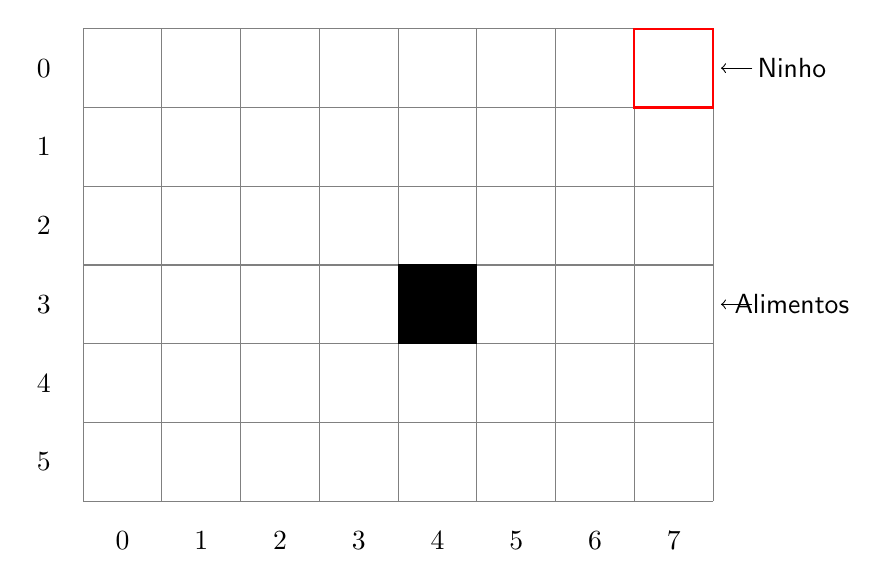
\begin{tikzpicture}
\draw[step=1cm,gray,thin] (0,0) grid (8,6);
\foreach \n/\x in {0/.5, 1/1.5, 2/2.5, 3/3.5, 4/4.5, 5/5.5, 6/6.5, 7/7.5}
  \node at (\x, -.5) {\p{\n}};
\foreach \n/\y in {5/.5, 4/1.5, 3/2.5, 2/3.5, 1/4.5, 0/5.5}
  \node at (-.5, \y) {\p{\n}};
\draw[fill] (4,2) rectangle +(1,1);
\node at (9,2.5) {\textsf{Alimentos}};
\draw[->] (8.5,2.5) to +(-.4,0);
\node at (9,5.5) {\textsf{Ninho}};
\draw[->] (8.5,5.5) to +(-.4,0);
\draw[red,thick] (7,5) rectangle +(1,1);
\end{tikzpicture}
\end{center}
\caption{Representação do meio ambiente como uma grade de células}\label{fig.ant-grid-empty}
\end{figure}

Sem qualquer informação sobre como as formigas escolhem seus movimentos, assumimos que elas podem se mover em qualquer direção com a mesma probabilidade, então a probabilidade de $p$ de uma formiga estar em qualquer célula é de $1$ dividido pelo número de células, aqui $p=1/48=0,021$.

A probabilidade de a formiga estar na célula com a fonte alimentar é de $p$, o mesmo que para qualquer outra célula. De acordo com nossa especificação do comportamento da formiga, uma vez que ela entra nesta célula e identifica a célula como a fonte de alimento, ela retorna diretamente ao ninho. Na Fig.~\ref{fig.ant-grid-empty} a fonte de alimento está na célula $(3,4)$, então uma formiga visitando essa célula deve retornar ao ninho na célula $(0,7)$, passando pelas células $(2,5)$ e $(1,6)$. Qual é a probabilidade de a formiga estar em qualquer uma destas três celas? Há duas possibilidades: ou a formiga está na célula porque se moveu aleatoriamente para lá com probabilidade de $p$, ou a formiga está lá porque se moveu para a fonte de alimento aleatoriamente com probabilidade de $p$ e depois \emph{com probabilidade de $1$} é movida para o ninho. Portanto, a probabilidade total de estar em qualquer uma dessas células é de $p+p\times 1=p+p=2p$.\footnote{Após as probabilidades serem atualizadas, elas devem ser normalizadas como explicado no Apêndice~\ref{a.normalize}. Para outro exemplo de normalização, veja Sect.~\ref{s.prob-local}.}  Se nosso robô está desenhando linhas à medida que se move, as células na diagonal devem ser duas vezes mais escuras do que as outras células.

\begin{figure}
\begin{center}
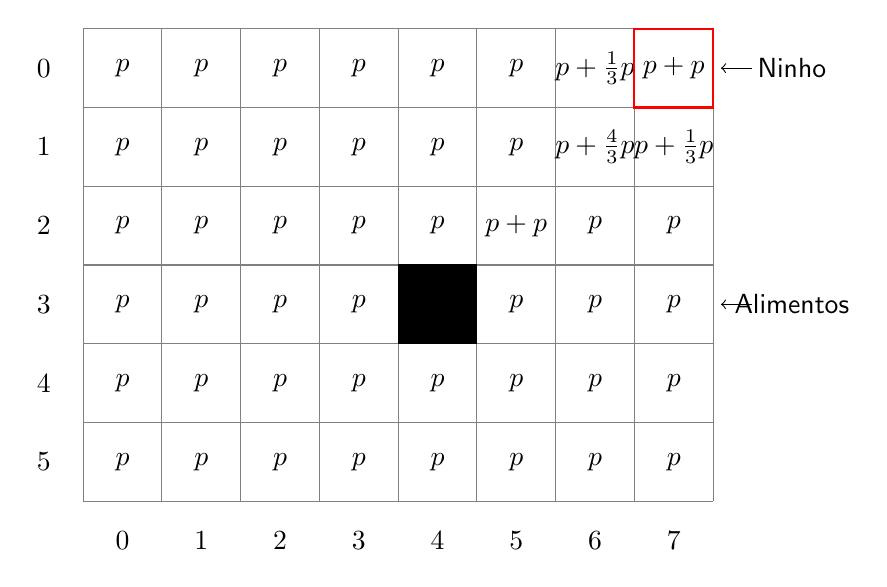
\begin{tikzpicture}
\draw[step=1cm,gray,thin] (0,0) grid (8,6);
\foreach \n/\x in {0/.5, 1/1.5, 2/2.5, 3/3.5, 4/4.5, 5/5.5, 6/6.5, 7/7.5}
  \node at (\x, -.5) {\p{\n}};
\foreach \n/\y in {5/.5, 4/1.5, 3/2.5, 2/3.5, 1/4.5, 0/5.5}
  \node at (-.5, \y) {\p{\n}};
\draw[fill] (4,2) rectangle +(1,1);
\node at (9,2.5) {\textsf{Alimentos}};
\draw[->] (8.5,2.5) to +(-.4,0);
\node at (9,5.5) {\textsf{Ninho}};
\draw[->] (8.5,5.5) to +(-.4,0);
\foreach \x in {.5, 1.5, 2.5, 3.5}
  \foreach \y in {.5, 1.5, 2.5, 3.5, 4.5, 5.5}
     \node at (\x,\y) {$p$};
\foreach \y in {.5, 1.5, 3.5, 4.5, 5.5}
     \node at (4.5,\y) {$p$};
\foreach \y in {.5, 1.5, 2.5, 4.5, 5.5}
     \node at (5.5,\y) {$p$};
\foreach \x in {6.5, 7.5}
  \foreach \y in {.5, 1.5, 2.5, 3.5}
     \node at (\x,\y) {$p$};
\node at (5.5,3.5) {$p+p$};
\node at (7.5,5.5) {$p+p$};
\node at (6.5,4.5) {$p+\frac{4}{3}p$};
\node at (7.5,4.5) {$p+\frac{1}{3}p$};
\node at (6.5,5.5) {$p+\frac{1}{3}p$};
\draw[red,thick] (7,5) rectangle +(1,1);
\end{tikzpicture}
\end{center}
\caption{Probabilidades para a localização da formiga}\label{fig.ant-grid-prob}
\end{figure}

\begin{figure}
\begin{center}
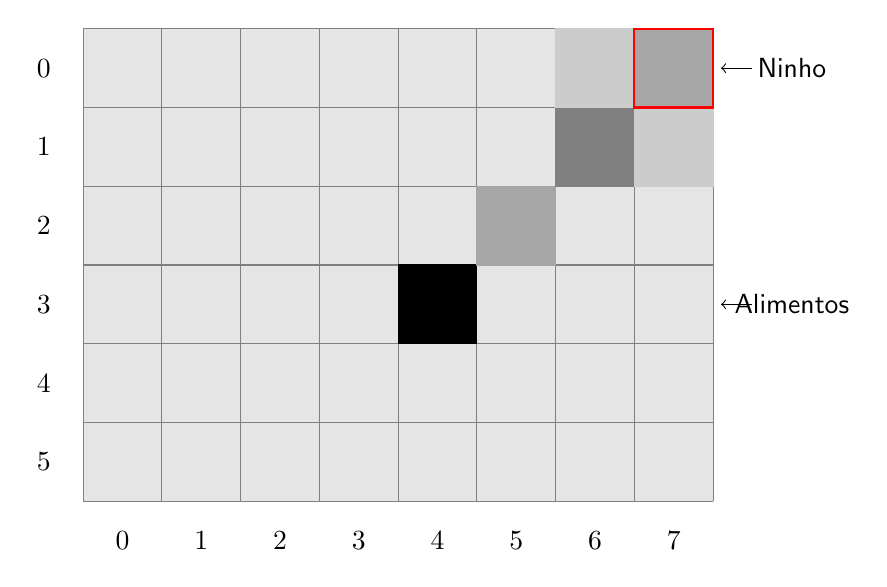
\begin{tikzpicture}
\node at (9,2.5) {\textsf{Alimentos}};
\draw[->] (8.5,2.5) to +(-.4,0);
\node at (9,5.5) {\textsf{Ninho}};
\draw[->] (8.5,5.5) to +(-.4,0);
\foreach \x in {0, 1, 2, 3, 4, 5, 6, 7}
  \foreach \y in {0, 1, 2, 3, 4, 5}
  \draw[fill,gray!20] (\x,\y) rectangle +(1,1);
\draw[step=1cm,gray,thin] (0,0) grid (8,6);
\draw[fill] (4,2) rectangle +(1,1);
\draw[fill,gray!70] (5,3) rectangle +(1,1);
\draw[fill,gray] (6,4) rectangle +(1,1);
\draw[fill,gray!70] (7,5) rectangle +(1,1);
\draw[fill,gray!40] (6,5) rectangle +(1,1);
\draw[fill,gray!40] (7,4) rectangle +(1,1);
\foreach \n/\x in {0/.5, 1/1.5, 2/2.5, 3/3.5, 4/4.5, 5/5.5, 6/6.5, 7/7.5}
  \node at (\x, -.5) {\p{\n}};
\foreach \n/\y in {5/.5, 4/1.5, 3/2.5, 2/3.5, 1/4.5, 0/5.5}
  \node at (-.5, \y) {\p{\n}};
\draw[red,thick] (7,5) rectangle +(1,1);
\end{tikzpicture}
\end{center}
\caption{Probabilidades para a localização de um robô com um marcador}\label{fig.ant-grid-gray}
\end{figure}

Uma vez que a formiga tenha alcançado o ninho, ela se moverá novamente de forma aleatória, ou seja, selecionará um vizinho aleatório para o qual se mover. Em geral, uma célula tem oito vizinhos (acima e abaixo, esquerda e direita, quatro nas diagonais), então a probabilidade é de $p/8$ de que ela esteja em qualquer um desses vizinhos. O ninho, entretanto, está no canto com apenas três vizinhos, então a probabilidade é de $p/3$ de que ele se moverá para qualquer um deles. A figura~\ref{fig.ant-grid-prob} mostra a probabilidade da localização da formiga após encontrar a fonte de alimento, retornando ao ninho e fazendo um movimento aleatório adicional. Quando implementadas por um robô com um marcador, as células com maior probabilidade se tornarão mais escuras (Fig.~\ref{fig.ant-grid-prob}).

O que podemos concluir a partir deste modelo?
\begin{itemize}
\item Embora as formigas se movam aleatoriamente, seu comportamento de retornar ao ninho após encontrar a fonte de alimento faz com que a probabilidade de estarem na diagonal seja maior do que em qualquer outra parte do ambiente. 
\item Como as formigas deixam cair feromonas (marcas pretas) em cada célula que visitam, segue-se que as marcas no caminho diagonal entre a fonte de alimento e o ninho serão mais escuras do que as marcas em outras células. Eventualmente, as marcas neste caminho serão suficientemente escuras para que o robô possa segui-las até a fonte de alimento sem realizar uma exploração aleatória.
\item Como o robô visita o ninho com freqüência, as células na vizinhança imediata do ninho terão uma probabilidade em algum lugar entre a probabilidade uniforme e a alta probabilidade da trilha. Portanto, é importante enfatizar a trilha usando métodos como os explorados em Activity~\ref{act.high-density}.
\end{itemize}

\section{Uma máquina de estado finito para o algoritmo de localização do caminho}\label{s.fsm-ants}

Um FSM para encontrar caminhos pelas formigas é mostrado na Fig.~\ref{fig.fsm-ant}. Para economizar espaço as etiquetas das transições usam abreviações que são explicadas na Tabela~\ref{tab.abbrev}. Aqui está uma descrição detalhada do comportamento especificado por este EFM em cada estado:

\smallskip

\begin{figure}
\begin{center}
\begin{tikzpicture}[node distance = 3.5cm and 4.9cm,align=left,minimum size=14mm,every loop/.style={min distance=16mm}]
% Nodes
\node[draw,circle] (search) {\p{search}};
\node[draw,circle] (follow) [right=of search] {\p{siga}};
\node[draw,circle] (food) [below=of follow] {\p{na alimentação}};
\node[draw,circle] (nest) [below=of search] {\p{ir para}\\\p{ninho}};
% Initial state arrow
\draw[->] (-15mm,10mm) to node [above left,xshift=6pt] {\p{verdadeiro} $\leadsto$ \p{fwd}} (search);
% Transitions from search
\path[->] (search) edge [loop left] node [below,yshift=-1mm] {\p{parede} $\leadsto$\\\p{turn $90$--$270$,}\\\p{fwd}} ();
\path[->] (search) edge [loop above] node {\p{timeout} $\leadsto$\\\p{giro $0$--$360$,}\\\p{fwd}} ();
\path[->,bend left=40] (search) edge node[above,xshift=-2mm,yshift=-3mm] {\p{cinza} $\leadsto$  \p{fwd}} (follow);
% Transitions from follow
\path[->] (follow) edge [loop above] node[yshift=-1mm] {\p{cinza R/L} $\leadsto$\\\p{fwd R/L}} ();
\path[->] (follow) edge [loop right] node [below,yshift=-1mm,xshift=-3mm] {\p{cinza R\&L} $\leadsto$\\\p{fwd}} ();
\path[->] (follow) edge node[above,yshift=-3mm] {\p{timeout} $\leadsto$ \p{fwd}} (search);
\path[->,bend left=15] (follow) edge node[left,yshift=4mm,xshift=17mm] {\p{preto} $\leadsto$ \p{--}} (food);
\path[->,bend left=40] (follow) edge node[below,xshift=4mm] {\p{parede} $\leadsto$\\\p{giro} $450$--$360$, \p{fwd}} (search);
% Transitions from at food
\path[->] (food) edge [loop right] node [below,yshift=-3mm,xshift=-2mm] {\p{direção do ninho}\\\p{não encontrado} $\leadsto$\\\p{girar}} ();
\path[->] (food) edge node[below,yshift=2mm] {\p{direção do ninho encontrado} $\leadsto$\\\p{virar para o ninho}} (nest);
% Transitions from nest
\path[->,bend left=15] (nest) edge node[right,xshift=-23mm,yshift=1mm] {\p{no ninho} $\leadsto$ \p{fwd}} (search);
\path[->] (nest) edge [loop left] node [above,yshift=1mm] {\p{ninho R/L} $\leadsto$\\\p{fwd R/L}} ();
\path[->] (nest) edge [loop below] node[left,xshift=-8mm,yshift=4mm] {\p{frente do ninho} $\leadsto$\\\p{fwd}} ();
\end{tikzpicture}
\end{center}
\caption{Máquina de estado para traçar um caminho entre uma fonte de alimento e um ninho\newline Veja a Tabela ~ref{tab.abbrev} para explicações sobre as abreviações}\label{fig.fsm-ant}
\end{figure}

\begin{table}[bt]
\caption{Abreviaturas na máquina estatal}
\label{tab.abbrev}
\begin{tabular}{p{2.5cm}p{8cm}}
\hline\noalign{\smallskip}
Abreviação & Explicação \\
\noalign{\smallskip}\hline\noalign{\smallskip}
\p{fwd} & \p{definir o motor para a frente}\\
\p{fwd R/L} & \p{colocar motor para a frente e para a direita/esquerda}\\
& \p{\bfseries fwd e fwd R/L também ajustam o temporizador para um período aleatório}\\
\p{parede} & \p{parede detectada}\\
\p{timeout} & \p{período de tempo expirado}\\
\p{cinza R/L/R\&L} & \p{cinza detectado pelos sensores direita/esquerda/ambos}\\
\p{frente do ninho/R/L} & \p{ninho detectado na frente/direita/esquerda}\\
\p{preto} & \p{preto detectado}\\
\p{direção do ninho} & \p{direção da comida ao ninho encontrado ou não encontrado}\\
\p{giro $\theta_1$--$\,\theta_2$} & \p{giram aleatoriamente na faixa $\theta_1$--$\,\theta_2$}\\
\p{girar}&\p{o robô (ou seu sensor) gira}\\
\noalign{\smallskip}\hline\noalign{\smallskip}
\end{tabular}
\end{table}

\noindent\textbf{\p{search}:} Neste estado, o robô procura aleatoriamente por áreas escuras. É o estado inicial e a transição \p{verdadeiro $\leadsto $ fwd} especifica que inicialmente (e incondicionalmente) o robô está se movendo para frente e um cronômetro é definido para um período aleatório. Quando o timer expira (tempo esgotado), o robô faz uma volta aleatória, move-se para frente e reinicia o timer. Este movimento aleatório continuará até que o robô encontre a parede da área ou uma marca cinza na superfície da área.  Uma vez que o robô tenha detectado uma marca cinzenta, ele faz a transição para o estado.

\smallskip

\noindent\textbf{\p{siga}:} As duas auto-transições acima e à direita deste estado são transições que implementam a linha seguinte (Sect.~ref{s.line}). Há três outras transições: Caso um \p{timeout} ocorra sem detectar o cinza, o robô não está mais seguindo uma linha e deve retornar ao estado de \p (busca). Se o robô encontrar uma parede, queremos que ele se afaste, mas primeiro pedimos que ele faça uma volta completa de $360^\circ$ para verificar se há uma marca de cinza em sua vizinhança. Portanto, a transição inclui a ação $450$--$360$. Como o ninho está ao lado de uma parede, esta condição também é verdadeira quando o robô retorna ao ninho. Se o robô sentir uma marcação de alta densidade (preto), ele conclui que alcançou a fonte de alimento e faz a transição para o estado de alimento.

\smallskip

\noindent\textbf{\p{na alimentação}:} Finalmente, o robô descobriu a fonte de alimentos. Agora ele deve voltar ao ninho. Nós especificamos que o ninho pode ser detectado (Activity~\ref{act.locate-nest}), mas o sensor do robô não necessariamente enfrenta a direção do ninho. Portanto, o robô (ou seu sensor) deve girar até encontrar a direção para o ninho. Quando o faz, ele se volta em direção ao ninho e faz a transição para o estado \p{goto ninho}.

\smallskip

\noindent\textbf{\p{goto nest}:} Este estado é semelhante ao estado {seguinte} em que o robô avança em direção ao ninho, virando à direita ou à esquerda conforme necessário para se mover na direção do ninho. Quando atinge o ninho, ele retorna ao estado de "pesquisa".

\smallskip

Veja novamente a Fig.~\ref{fig.ant-result} que mostra uma experiência real com um robô rodando este algoritmo. Vemos que há uma alta densidade de linhas entre o ninho e a fonte de alimento, mas também há uma densidade relativamente alta de linhas nas proximidades do ninho, não necessariamente na direção da fonte de alimento. Isto pode fazer com que o robô volte à busca aleatória em vez de ir diretamente para a fonte de alimento.

\section{Sumário}

Os algoritmos para evitar obstáculos utilizam muros seguindo algoritmos que são conhecidos desde tempos antigos no contexto da navegação em um labirinto. Quando usado para evitar obstáculos, várias anomalias podem fazer com que os algoritmos falhem, em particular, o obstáculo em forma de $G$ pode aprisionar uma parede seguindo o algoritmo. O algoritmo Pledge supera esta dificuldade.

Uma colônia de formigas pode determinar um caminho entre seu ninho e uma fonte de alimento sem saber sua localização e sem um mapa, reforçando um comportamento aleatório que tem um resultado positivo.

\section{Leitura adicional}

Há uma grande literatura sobre labirintos que pode ser encontrada seguindo as referências no artigo da Wikipedia para \emph{Maze}. O algoritmo Pledge foi descoberto por John Pledge, de 12 anos; nossa apresentação é baseada em \cite[Cap.~4]{turtle}. Um projeto baseado em formigas seguindo feromonas é descrito em~\cite{Mayet2010}.
